\documentclass[]{article}
\usepackage[a4paper]{geometry}
\usepackage[dutch]{babel}
% Floating figuren.
\usepackage{graphicx}

% Mooie captions en subfiguren.
\usepackage{caption}
\usepackage{subcaption}

\usepackage{titling}

% Om code en dergelijke te plaatsen.
\usepackage{listings}

% Wiskundige formules in LaTeX <3
\usepackage{amsmath}
\usepackage{amssymb}
\usepackage{amsfonts}

% MATRICES! :D
\usepackage{amsmath}
\setcounter{MaxMatrixCols}{25}

% Ik vind het nu eenmaal mooier zo.
\setlength{\parindent}{0pt}
\setlength{\parskip}{14pt}
\setlength{\droptitle}{-9em}

\title{Project Datacommunicatie}
\author{Enver Bral \\
        Fr\'ed\'erique De Baerdemaeker \\
        Ruben Taelman \\
        Felix Van der Jeugt}
\date{Academiejaar 2012 - 2013}

\begin{document}

\maketitle
\begin{section}*{Broncodering}

    \begin{subsection}*{Vraag 1}

        We verkrijgen volgende output bij het uitvoeren van
        \texttt{FrequencyCounter.m}:

        \begin{lstlisting}
            0.5443    0.0024    0.0031    0.0040
            0.0019    0.0045    0.0001    0.0026
            0.0020    0.0001    0.0044    0.0029
            0.0045    0.0025    0.0018    0.4189
        \end{lstlisting}

        Dit zijn de relatieve frequenties voor elk macroblok. De
        macroblokken zijn hier als volgt genummerd: We zetten de rijen
        van het macroblok na elkaar, en lezen ze als een binair getal.  Zo
        wordt het macroblock \texttt{[1 0;0 1]} omgezet naar
        \texttt{1 0 0 1} en krijgt het nummer $9$.

        Met deze frequenties kunnen we de Huffman-boom opstellen. Deze
        vindt u in Figuur~\ref{fig:manual_huffman}. Door aan de
        vertakking met het kleinste deelgewicht een nul toe te kennen,
        en een \'e\'en anders, bekomen we de codering in
        Tabel~\ref{tab:manual_huffman}.

        \begin{figure}
            \centering
            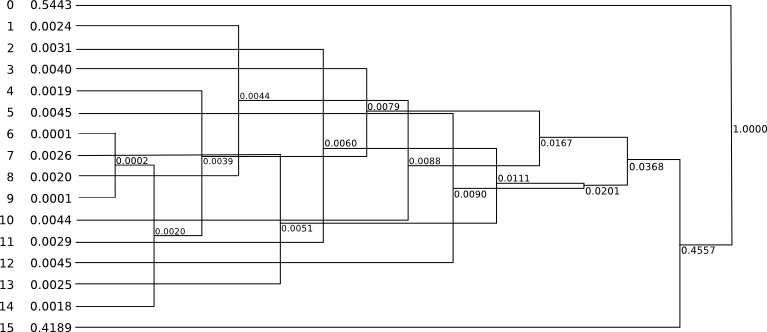
\includegraphics[width=\textwidth]{manual_huffman.png}
            \caption{Huffmanboom, opgesteld bij de frequenties uit
            \label{fig:manual_huffman}
            vraag 1.}
        \end{figure}

        \begin{table}
            \centering
            \begin{tabular}{lr@{.}lr}
                \textbf{Macrosymbool} &
                \multicolumn{2}{l}{\textbf{Rel. freq.}} &
                \textbf{Codewoord} \\
                \hline
                \texttt{0000} & 54 & 43 \% & \texttt{1} \\
                \texttt{0001} &  0 & 24 \% & \texttt{000101} \\
                \texttt{0010} &  0 & 31 \% & \texttt{001111} \\
                \texttt{0011} &  0 & 40 \% & \texttt{00001} \\
                \texttt{0100} &  0 & 19 \% & \texttt{000000} \\
                \texttt{0101} &  0 & 45 \% & \texttt{00100} \\
                \texttt{0110} &  0 & 01 \% & \texttt{00000100} \\
                \texttt{0111} &  0 & 26 \% & \texttt{001101} \\
                \texttt{1000} &  0 & 20 \% & \texttt{000100} \\
                \texttt{1001} &  0 & 01 \% & \texttt{00000101} \\
                \texttt{1010} &  0 & 44 \% & \texttt{00011} \\
                \texttt{1011} &  0 & 29 \% & \texttt{001110} \\
                \texttt{1100} &  0 & 45 \% & \texttt{00101} \\
                \texttt{1101} &  0 & 25 \% & \texttt{001100} \\
                \texttt{1110} &  0 & 18 \% & \texttt{0000011} \\
                \texttt{1111} & 41 & 89 \% & \texttt{01} \\
            \end{tabular}
            \caption{De Huffmancode bij vraag 1.}
            \label{tab:manual_huffman}
        \end{table}

        Nu kunnen we het gemiddeld aantal codebits per bronsymbool
        eenvoudig berekenen:

        \begin{eqnarray*}
            \mathbb{E}(n)
            &=& \frac{1}{4} \sum^{16}_{i=1}{p_i c_i} \\
            &=& \frac{1}{4*100}(1*54.43 + 6*0.24 + 6*0.31 + 5*0.40
                + 6*0.19 + 5*0.45 + 8*0.01 \\ && + 6*0.26 + 6*0.20
                + 8*0.01 + 5*0.44 + 6*0.29 + 5*0.45 + 6*0.25 \\ &&
                + 7*0.18 + 2*41.89) \\
            &=& \frac{158.77}{400} \\
            &=& 0.396925
        \end{eqnarray*}

        De afbeelding kan dus tot amper 40 procent van zijn
        oorspronkelijke grootte gereduceerd worden met behulp van
        Huffmancodering.

    \end{subsection}

    \begin{subsection}*{Vraag 3}

        We verkrijgen grafiek~\ref{fig:vraag1_3} bij het uitvoeren van \texttt{vraag1\_3.m}:

        % TODO figure environment and caption.
        \begin{figure}[h]
            \centering
            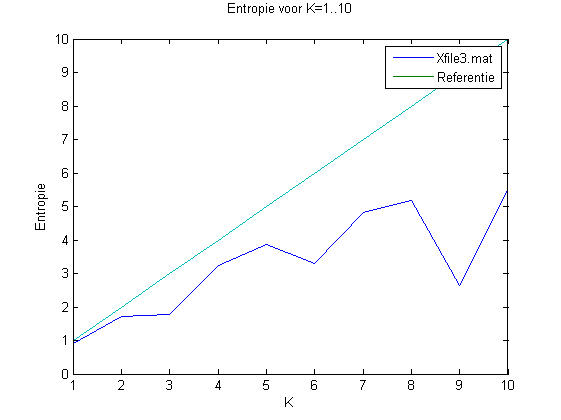
\includegraphics[width=\textwidth]{vraag1_3.png}
            \caption{Gemiddeld aantal codebits per bronsymbool}
            \label{fig:vraag1_3}
        \end{figure}

        In grafiek~\ref{fig:vraag1_3} kunnen we de entropie zien van de macrosymbolen van
        grootte K. De referentielijn is hier een rechte, dit is logisch
        aangezien de entropie maximaal is wanneer alle symbolen met
        gelijke kans voorkomen.
        Over het algemeen stijgt de entropie bij een grotere K, behalve
        bij K=6 en K=9.

    \end{subsection}

    \begin{subsection}*{Vraag 4}

	Door \texttt{vraag1\_4.main()} bekomen we het resultaat te zien op figuur \ref{fig:codebits}.
	Hierop kunnen we het gemiddelde aantal codebits per bronsymbool
        (gebruikmakend van Huffman-codering) voor macrosymbolen met
        grootte K=1..10 en de bijhorende onder/bovengrens zien.
        \begin{figure}[h]
            \centering
            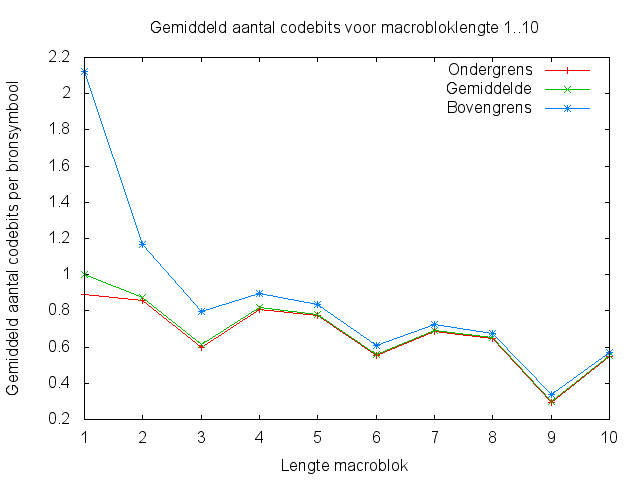
\includegraphics[width=\textwidth]{vraag1_4.png}
            \caption{Gemiddeld aantal codebits per bronsymbool}
            \label{fig:codebits}
        \end{figure}

        Als ondergrens nemen we de entropie van een bronsymbool
        \textbf{H(X)} en als bovengrens nemen we
        $\mathbf{H(X) +\frac{1}{K}}$.

        We vinden dat het bestand het best gecomprimeerd is voor
        \textbf{K=9} met \textbf{0.2982} codebits per bronsymbool. Dit
        is eveneens de compressiefactor. Het kan misschien  interessant
        zijn om bijvoorbeeld \textbf{K=3} of \textbf{K=6} te gebruiken
        naargelang uitvoertijd van belang is. Voor deze
        macroblok-groottes duurt het immers minder lang om een codeboek
        op te stellen.
		
    \end{subsection}

    \begin{subsection}*{Vraag 5}

        In Figuur~\ref{fig:codebits} zien we dat $\mathbb{E}[n]$ zeer
        dicht bij de ondergrens ligt. Enkel voor macroblokken van
        grootte \'e\'en is dit niet het geval, maar aangezien we geen
        codewoorden van minder dan \'e\'en bit kunnen toekennen, is dit
        slechts te verwachten. Dit kleine verschil wijst erop dat
        Huffman-codering een zeer goede broncodering is.

        We vragen ons nu af, of het mogelijk is om de ondergrens te
        bereiken met huffmancodering. Met andere woorden, wanneer zal
        $H(x) = E[n]$:

        \begin{eqnarray*}
            H(x) = E[n]
            & \Leftrightarrow & - \sum_{x \in A}{p(x) \log_2{p(x)}}
                = \frac{1}{K} \sum_{i = 1}^{N}{p_i n_i}
        \end{eqnarray*}

        Nu zal de verzameling $A$ die van alle macrowoorden zijn,
        wat ons brengt tot:

        \begin{eqnarray*}
            H(x) = E[n]
            & \Leftrightarrow & - \sum_{i = 1}^{N}{p_i \log_2{p_i}}
                = \frac{1}{K} \sum_{i = 1}^{N}{p_i n_i} \\
            & \Leftrightarrow & \sum_{i = 1}^{N}(p_i \log_2{p_i}
                + \frac{p_i n_i}{K}) = 0 \\
            & \Leftrightarrow & \sum_{i = 1}^{N}(
                \frac{K p_i \log_2{p_i} + p_i n_i}{K}) = 0 \\
            & \Leftrightarrow & \sum_{i = 1}^{N}(K \log_2{p_i} + n_i)
                = 0
        \end{eqnarray*}

        De enige term die hierin negatief kan zijn, is het logaritme.
        Bijgevolg:

        \begin{eqnarray*}
            H(x) = E[n] & \Leftrightarrow &
            \sum_{i = 1}^{N}K \log_2{p_i} = - \sum_{i = 1}^{N} n_i
            \\ & \Leftrightarrow &
            K \log_2 {\prod_{i = 1}^{N}{\frac{1}{p_i}}}
                = \sum_{i = 1}^{N} n_i
        \end{eqnarray*}

        Aldus hebben we de voorwaarden bepaald, waaronder de
        Huffman-codering de ondergrens kan bereiken. Nu, omdat de som
        van de kansen $p_i$ steeds $1$ zal zijn, zijn beide leden nu
        positief. We plotten de mogelijke ranges in functie van N.

        De minimale waarde van het linkerlid wordt bereikt wanneer het
        product minimaal is, en dat is wanneer alle $p_i$ even groot
        zijn. Formule: $\min(LL) = K \log_2{N^N} = KN \log_2{N}$. De
        maximale waarde voor het linkerlid is uiteraard oneindig, als
        \'e\'en van de woorden niet voorkomt: $ \max(LL) = K*log_2{0}
        = \infty $.

        Als we nu eens enkele eenvoudige gevallen voor het rechterlid
        bekijken:

        \begin{itemize}
            \item We kunnen bijvoorbeeld alle macrowoorden van gelijke
                frequentie nemen. Dan bekomen we een complete binaire
                boom als Huffmanboom. Deze heeft uiteraard een diepte
                van $\log_2 N$ in al zijn paden, dus we krijgen als
                rechterlid $N \log_2 N$.

                In dit geval zal de Huffmancode enkel optimaal zijn als
                $K$ gelijk is aan 1. Natuurlijk is 1 een vrij
                belachelijke waarde voor K.
            \item We kunnen ook werken met $n_1 = 1$ en $(\forall i>1)
                (n_i = 2^{i-1})$. De gevormde boom zal eerst $n_1$ en
                $n_2$ samennemen, en dan telkens alle voorgaande, en
                een nieuw getal. Zodanig zullen de paden naar de toppen
                alle natuurlijke getallen tot $N$ bevatten. Hun som
                moet dan groter zijn dan ons linkerlid:
                \begin{eqnarray*}
                    N + \frac{N(N+1)}{2} \ge K N \log_2 N
                    \\ & \Leftrightarrow &
                    N^2 + 3N \ge 2KN \log_2 N
                    \\ & \Leftrightarrow &
                    N + 3 \ge 2K \log_2 N
                \end{eqnarray*}
                Uiteraard zal K meestal zeer groot zijn, maar voor
                grotere alfabetten zal de Huffmancode optimaal blijken.
        \end{itemize}

    \end{subsection}

    \begin{subsection}*{Vraag 6}

        Vertrekkende van de \emph{niet-canonische} Huffmancode in
        Tabel~\ref{tab:manual_huffman}, vinden we de canonische
        Huffmancode gegeven in Tabel~\ref{tab:canonical_huffman}

        \begin{table}
            \centering
            \begin{tabular}{c|r}
                \textbf{Macrosymbool} &
                \textbf{Codewoord} \\
                \hline
                \texttt{0000} & \texttt{0} \\
                \texttt{0001} & \texttt{111000} \\
                \texttt{0010} & \texttt{111001} \\
                \texttt{0011} & \texttt{11000} \\
                \texttt{0100} & \texttt{111010} \\
                \texttt{0101} & \texttt{11001} \\
                \texttt{0110} & \texttt{11111110} \\
                \texttt{0111} & \texttt{111011} \\
                \texttt{1000} & \texttt{111100} \\
                \texttt{1001} & \texttt{11111111} \\
                \texttt{1010} & \texttt{11010} \\
                \texttt{1011} & \texttt{111101} \\
                \texttt{1100} & \texttt{11011} \\
                \texttt{1101} & \texttt{111110} \\
                \texttt{1110} & \texttt{1111110} \\
                \texttt{1111} & \texttt{10} \\
            \end{tabular}
            \caption{Canonische Huffmancode bij vraag 6}
            \label{tab:canonical_huffman}
        \end{table}

    \end{subsection}

    \begin{subsection}*{Vraag 7}
        Na het toepassen van het algoritme om een alfabet om te zetten
        naar een canonische Huffmancode bekomen we het resultaat in
        Tabel~\ref{tab:canonical_codes}.

        \begin{table}
            \centering
            \begin{tabular}{c|c}
            \textbf{Letter} &
            \textbf{Codewoord} \\
            D & 0 \\
            B & 100 \\
            C & 101 \\
            G & 110 \\
            E & 1110 \\
            A & 11110 \\
            F & 11111 \\
            \end{tabular}
            \caption{De codewoorden bij vraag 7 in canonische vorm}
            \label{tab:canonical_codes}
        \end{table}

    \end{subsection}

\end{section}
\newpage
\begin{section}*{Kanaalcodering}

    \begin{subsection}*{Vraag 1}
        Onze generatorveelterm is $g(x) = x^4 + x + 1$.

        Als minimale Hamming-afstand voor de gegeven code bekomen we
        $d=3$. Hiermee kunnen we het fout-detecterend en corrigerend
        vermogen berekenen als volgt:
        \begin{eqnarray*}
            & \text{fout-detecterend vermogen} = d-1 = 2 \\
            & \text{fout-corrigerend vermogen} = floor((d-1)/2) = 1
        \end{eqnarray*}

        De checkveelterm kunnen we bepalen aan de hand van volgende
        vergelijking:
        \begin{eqnarray*}
            x^{15} + 1 &=& h(x) * g(x)
        \end{eqnarray*}

        We weten al $g(x)$, dus we kunnen met behulp van een
        Euclidische deling $h(x)$ zoeken. We bekomen:
        \begin{eqnarray*}
            h(x) &=& x^{11} + x^8 + x^7 + x^5 + x^3 + x^2 + x + 1
        \end{eqnarray*}

        Als de matrices bekomen we:
        \[
            G =\begin{pmatrix}
1 & 1 & 0 & 0 & 1 & 0 & 0 & 0 & 0 & 0 & 0 & 0 & 0 & 0 & 0 \\
0 & 1 & 1 & 0 & 0 & 1 & 0 & 0 & 0 & 0 & 0 & 0 & 0 & 0 & 0 \\
0 & 0 & 1 & 1 & 0 & 0 & 1 & 0 & 0 & 0 & 0 & 0 & 0 & 0 & 0 \\
0 & 0 & 0 & 1 & 1 & 0 & 0 & 1 & 0 & 0 & 0 & 0 & 0 & 0 & 0 \\
0 & 0 & 0 & 0 & 1 & 1 & 0 & 0 & 1 & 0 & 0 & 0 & 0 & 0 & 0 \\
0 & 0 & 0 & 0 & 0 & 1 & 1 & 0 & 0 & 1 & 0 & 0 & 0 & 0 & 0 \\
0 & 0 & 0 & 0 & 0 & 0 & 1 & 1 & 0 & 0 & 1 & 0 & 0 & 0 & 0 \\
0 & 0 & 0 & 0 & 0 & 0 & 0 & 1 & 1 & 0 & 0 & 1 & 0 & 0 & 0 \\
0 & 0 & 0 & 0 & 0 & 0 & 0 & 0 & 1 & 1 & 0 & 0 & 1 & 0 & 0 \\
0 & 0 & 0 & 0 & 0 & 0 & 0 & 0 & 0 & 1 & 1 & 0 & 0 & 1 & 0 \\
0 & 0 & 0 & 0 & 0 & 0 & 0 & 0 & 0 & 0 & 1 & 1 & 0 & 0 & 1 \\
\end{pmatrix}
\\
        \]\[
            H =\begin{pmatrix}
1 & 1 & 1 & 1 & 0 & 0 & 0 & 0 & 0 & 0 & 0 & 0 & 0 & 0 & 0 \\
0 & 1 & 1 & 1 & 1 & 0 & 0 & 0 & 0 & 0 & 0 & 0 & 0 & 0 & 0 \\
0 & 0 & 1 & 1 & 1 & 1 & 0 & 0 & 0 & 0 & 0 & 0 & 0 & 0 & 0 \\
0 & 0 & 0 & 1 & 1 & 1 & 1 & 0 & 0 & 0 & 0 & 0 & 0 & 0 & 0 \\
0 & 0 & 0 & 0 & 1 & 1 & 1 & 1 & 0 & 0 & 0 & 0 & 0 & 0 & 0 \\
0 & 0 & 0 & 0 & 0 & 1 & 1 & 1 & 1 & 0 & 0 & 0 & 0 & 0 & 0 \\
0 & 0 & 0 & 0 & 0 & 0 & 1 & 1 & 1 & 1 & 0 & 0 & 0 & 0 & 0 \\
0 & 0 & 0 & 0 & 0 & 0 & 0 & 1 & 1 & 1 & 1 & 0 & 0 & 0 & 0 \\
0 & 0 & 0 & 0 & 0 & 0 & 0 & 0 & 1 & 1 & 1 & 1 & 0 & 0 & 0 \\
0 & 0 & 0 & 0 & 0 & 0 & 0 & 0 & 0 & 1 & 1 & 1 & 1 & 0 & 0 \\
0 & 0 & 0 & 0 & 0 & 0 & 0 & 0 & 0 & 0 & 1 & 1 & 1 & 1 & 0 \\
\end{pmatrix}
\\
        \]\[
            G_{sys} =\begin{pmatrix}
1 & 0 & 0 & 0 & 0 & 0 & 0 & 0 & 0 & 0 & 0 & 1 & 1 & 0 & 0 \\
0 & 1 & 0 & 0 & 0 & 0 & 0 & 0 & 0 & 0 & 0 & 0 & 1 & 1 & 0 \\
0 & 0 & 1 & 0 & 0 & 0 & 0 & 0 & 0 & 0 & 0 & 0 & 0 & 1 & 1 \\
0 & 0 & 0 & 1 & 0 & 0 & 0 & 0 & 0 & 0 & 0 & 1 & 1 & 0 & 1 \\
0 & 0 & 0 & 0 & 1 & 0 & 0 & 0 & 0 & 0 & 0 & 1 & 0 & 1 & 0 \\
0 & 0 & 0 & 0 & 0 & 1 & 0 & 0 & 0 & 0 & 0 & 0 & 1 & 0 & 1 \\
0 & 0 & 0 & 0 & 0 & 0 & 1 & 0 & 0 & 0 & 0 & 1 & 1 & 1 & 0 \\
0 & 0 & 0 & 0 & 0 & 0 & 0 & 1 & 0 & 0 & 0 & 0 & 1 & 1 & 1 \\
0 & 0 & 0 & 0 & 0 & 0 & 0 & 0 & 1 & 0 & 0 & 1 & 1 & 1 & 1 \\
0 & 0 & 0 & 0 & 0 & 0 & 0 & 0 & 0 & 1 & 0 & 1 & 0 & 1 & 1 \\
0 & 0 & 0 & 0 & 0 & 0 & 0 & 0 & 0 & 0 & 1 & 1 & 0 & 0 & 1 \\
\end{pmatrix}
\\
        \]\[
            H_{sys} =\begin{pmatrix}
1 & 0 & 0 & 1 & 1 & 0 & 1 & 0 & 1 & 1 & 1 & 1 & 0 & 0 & 0 \\
1 & 1 & 0 & 1 & 0 & 1 & 1 & 1 & 1 & 0 & 0 & 0 & 1 & 0 & 0 \\
0 & 1 & 1 & 0 & 1 & 0 & 1 & 1 & 1 & 1 & 0 & 0 & 0 & 1 & 0 \\
0 & 0 & 1 & 1 & 0 & 1 & 0 & 1 & 1 & 1 & 1 & 0 & 0 & 0 & 1 \\
\end{pmatrix}

        \]

    \end{subsection}

    \begin{subsection}*{Vraag 2} % Jimmy

        We bepalen de syndroomtabel met behulp van de coset-leiders.
        In het totaal zijn er 16 ($2^{n-k}$) syndromen. We kunnen snel
        de coset-leiders bepalen door een nulrij en daaronder een
        eenheidsmatrix te plaatsen. Er is 1 coset-leider met gewicht
        0 en 15 coset-leiders met gewicht 1. We vermenigvuldigen nu
        deze coset-leiders met de getransponeerde checkmatrix uit de
        vorige vraag en bekomen zo de syndromen.

        \begin{table}
            \centering
            \begin{tabular}{@{}c|c@{}}
                Syndroom & Coset-leider \\
                \hline
                0000 & 000000000000000 \\
                1100 & 100000000000000 \\
                0110 & 010000000000000 \\
                0011 & 001000000000000 \\
                1101 & 000100000000000 \\
                1010 & 000010000000000 \\
                0101 & 000001000000000 \\
                1110 & 000000100000000 \\
                0111 & 000000010000000 \\
                1111 & 000000001000000 \\
                1011 & 000000000100000 \\
                1001 & 000000000010000 \\
                1000 & 000000000001000 \\
                0100 & 000000000000100 \\
                0010 & 000000000000010 \\
                0001 & 000000000000001
            \end{tabular}
            \caption{Syndroomtabel voor de cyclische (15,11)
            Hammingcode}
        \end{table}

        De kans op de een decodeerfout na een transmissie over een BSC
        met bitfoutprobabiliteit $p$ is
        \begin{eqnarray}
            Pr[\text{decodeerfout}] &=&1-Pr[\text{geen decodeerfout}]
                \nonumber \\
            &=&1-Pr[\textbf{e} \in \text{syndroomtabel}] \nonumber \\
            &=&1- ((1-p)^{15} + 15p(1-p)^{14}) \label{eqn:2_2}
        \end{eqnarray}

        Met het binomium van Newton kunnen we dit herleiden tot:
        \begin{eqnarray*}
            =&&(\sum_{i=0}^{15}(^{15}_i)p^i(1-p)^{n-i})- (1-p)^{15} -
                15p(1-p)^{14} \\
            =&& 105p^{2}(1-p)^{13} + 455p^{3}(1-p)^{12} +
                1365p^{4}(1-p)^{11}  + 3003p^{5}(1-p)^{10} \\
             &+& 5005p^{6}(1-p)^{9} + 6435p^{7}(1-p)^{8} +
                6435p^{8}(1-p)^{7} + 5005p^{9}(1-p)^{6} \\
             &+& 3003p^{10}(1-p)^{5} + 1365p^{11}(1-p)^{4} +
                455p^{12}(1-p)^{3} + 105p^{13}(1-p)^{2} \\
             &+& 15p^{14}(1-p) +p^{15}
        \end{eqnarray*}

        Voor $p << 1$ (zeer kleine waarden) kan dit benaderd worden
        met $105p^2$

    \end{subsection}

    \begin{subsection}*{Vraag 3} % Felix
        In \texttt{vraag2\_3.m} vindt u de code terug waarmee de
        simulaties uitgevoerd worden. Deze maakt gebruik van een
        ``vals'' kanaal dat bitfouten van kans $p$ introduceert. In
        tabel \ref{tab:2_3} vindt u de door simulatie gevonden
        kans op decodeerfouten in vergelijking met de theoretisch verwachte
        kans op fouten. De theoretische probabiliteit werd
        berekend met formule \ref{eqn:2_2}.

        Een grafische voorstelling van deze decodeerfouten vindt u in
        figuur \ref{fig:2_3}.

        \begin{table}
            \centering
            \begin{tabular}{rrr}
                \textbf{Foutprobabiliteit} &
                \textbf{Theoretisch} &
                \textbf{Re\"eel} \\
                $3 * 10^{-1}$ & 96.47 \% & 96.48 \% \\
                $1 * 10^{-1}$ & 45.09 \% & 45.60 \% \\
                $3 * 10^{-2}$ &  7.30 \% &  9.34 \% \\
                $1 * 10^{-2}$ &  0.96 \% &  0.55 \% \\
                $3 * 10^{-3}$ &  0.09 \% &  0.00 \% \\
                $1 * 10^{-3}$ &  0.01 \% &  0.00 \%
            \end{tabular}
            \caption{De theoretische en re\"ele kans op een fout
                gedecodeerd codewoord. De re\"ele kans werd bepaald
                door 10000 bits te verzenden, na het coderen met
            Hamming codering.}
            \label{tab:2_3}
        \end{table}

        \begin{figure}[h]
            \centering
            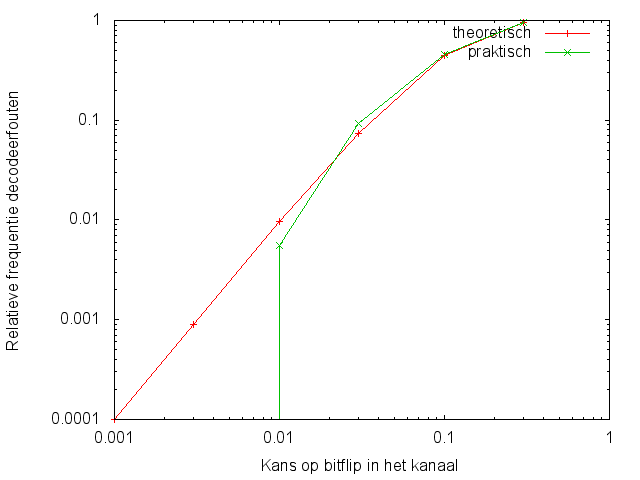
\includegraphics[width=0.8\textwidth]{vraag2_3.png}
            \caption{De theoretische en re\"ele decodeerfouten in
                functie van de foutprobabiliteit van het gebruikte
            kanaal.}
            \label{fig:2_3}
        \end{figure}

    \end{subsection}

    \begin{subsection}*{Vraag 4} % Enver
    	De minimale hammingafstand van de product code is het product van de minimale hammingafstand
van enerzijds de hamming code, zijnde 3, en anderzijds de minimale hammingafstand van de code waarbij we een pariteitsbit toevoegen, dewelke 2 is.
De minimale hammingafstand van de product code bedraagt dus 6.
    \end{subsection}

    \begin{subsection}*{Vraag 5} % Ruben

        Als er een even aantal (groter dan 2) syndromen verschillend
        zijn van de nulvector, dan weten wij dat de pariteitsbit
        juist staan, maar wij weten dan niet hoe we de fouten moeten
        corrigeren. Dit geval staat ook niet in de ge\"implementeerde
        code, dus deze soorten fouten zullen niet verbeterd worden.
        Een tweede geval waarbij er fout gecorrigeerd kan worden is
        wanneer er een fout optreed in de laatste rij van een blok, de
        pariteitsbits. Wanneer op deze positie ook in een bepaalde rij
        een van nul verschillend syndroom voorkomt dan kan het zijn
        dat een fout op de verkeerde manier hersteld zal worden.

    \end{subsection}

    \begin{subsection}*{Vraag 6} % Jimmy
        We vergelijken nu de kans dat er minimum 1 codewoord in een
        blok van 8 codewoorden fout gedecodeerd wordt met de gemeten
        kans op een decodeerfout bij de productcode. We kunnen deze
        kans analytisch als volgt berekenen:
        \begin{eqnarray*}
            Pr[\text{decodeerfout}]
                &=& 1 - Pr[\text{geen decodeerfout}]^8 \\ 
                &=& 1 - ((1-p)^{15} + 15p(1-p)^{14})^8
        \end{eqnarray*}

        We simuleren nu coderen en decoderen met productcode voor een
        willekeurige bit-sequentie van 10000 woorden lang en zoeken de
        fouten in vectoren van 88 bits (8 blokken x 11 bits per woord).
        
        De resultaten van \texttt{vraag2\_6.m} vinden we in tabel
        \ref{tab:2_6} en figuur \ref{fig:2_6}.

        \begin{table}[h]
            \centering	
            \begin{tabular}{r|r|r}
                Bitfoutprobabiliteit $p$ &
                Analytische kans (\%) &
                Gemeten kans (\%)\\
                \hline
                0.3   & 100    & 100   \\
                0.1   &  99.17 & 98.96 \\
                0.03  &  45.46 & 30.56 \\
                0.01  &   7.45 & 2.48  \\
                0.003 &   0.73 & 0.08  \\
                0.001 &   0.08 & 0
            \end{tabular}
            \caption{Vergelijking analytische met gemeten resultaat
            voor kans op een decodeerfout bij productcode.}
            \label{tab:2_6}
        \end{table}    
        \begin{figure}
            \centering
            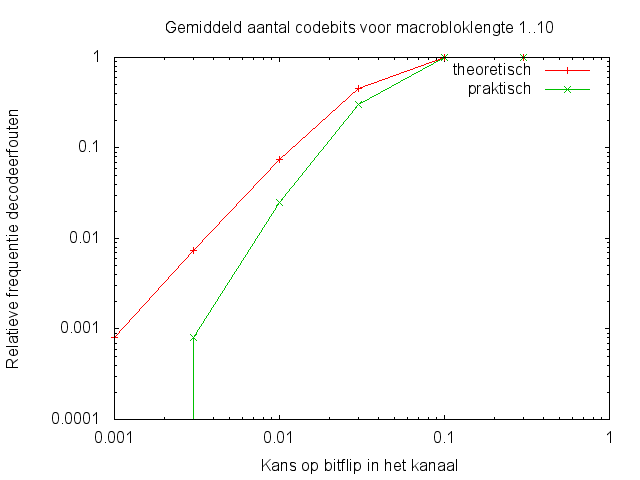
\includegraphics[width=0.7\textwidth]{vraag2_6.png}
            \caption{De theoretische en re\"ele kans op een
            decodeerfout voor de productcode}
            \label{fig:2_6}
        \end{figure}
    \end{subsection}
	
    \begin{subsection}*{Vraag 7} % Felix

        De figuren waarin de toekomende bits resulteren vindt u terug
        in figuur \ref{fig:2_7}.

        Wat de ongecodeerde transmissie betreft, is de verklaring niet
        ver te zoeken. Bij benadering is gewoon 1 op de 100 bits fout.
        Daardoor krijgen we een ``bespikkelde'' afbeelding.

        Bij de twee andere transmissies zijn de foute bits niet zomaar
        verdeeld. We zien duidelijk de fout gedecodeerde codewoorden
        zitten in verticale lijntjes van 11 bits lang. Bij figuur
        \ref{fig:ham_coded} (Hammingcode) zijn dit er een stuk
        meer dan bij figuur \ref{fig:prod_coded} (Product codering).

        Laat ons nu nog opmerken dat de fout gedecodeerde woorden
        willekeurig over de figuur verdeeld zijn. Daaruit kunnen we
        afleiden dat elk woord een even grote kans maakt om verkeerd
        ontvangen te worden.
        \begin{figure}[h]
            \centering
            \begin{subfigure}{0.24\textwidth}
                \centering
                
\includegraphics[width=\textwidth]{darthvader.png}
                \caption{}
                \label{fig:darthvader}
            \end{subfigure}
            \begin{subfigure}{0.24\textwidth}
                \centering
                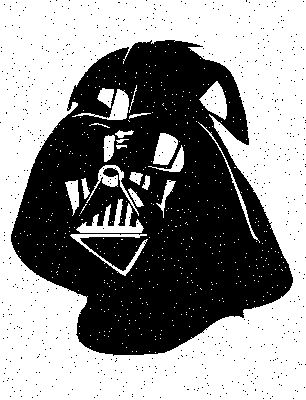
\includegraphics[width=\textwidth]{uncoded.png}
                \caption{}
                \label{fig:uncoded}
            \end{subfigure}
            \begin{subfigure}{0.24\textwidth}
                \centering
                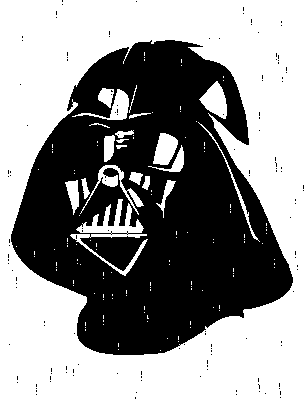
\includegraphics[width=\textwidth]{ham_coded.png}
                \caption{}
                \label{fig:ham_coded}
            \end{subfigure}
            \begin{subfigure}{0.24\textwidth}
                \centering
                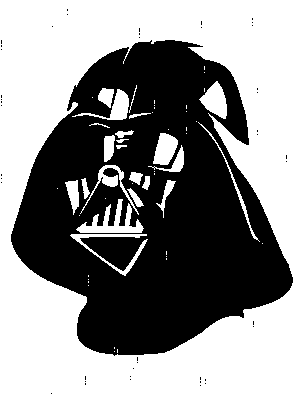
\includegraphics[width=\textwidth]{prod_coded.png}
                \caption{}
                \label{fig:prod_coded}
            \end{subfigure}

            \caption{De figuren bij vraag 2.7. Ter referentie ziet u in
                figuur (\ref{fig:darthvader}) de originele figuur. De
                drie daaropvolgende figuren tonen in volgorde de
                ongecodeerde, Hamming-gecodeerde en Product-gecodeerde
            transmissies.}

            \label{fig:2_7}

        \end{figure}
    \end{subsection} 
\end{section}
\clearpage
\begin{section}*{Volledig systeem} % Enver

	De resultaten van het doorsturen van de figuur over het kanaal zijn te zien
	in figuur~\ref{fig:3_3}.
	
	\par
	
	Wanneer we de afbeelding door het kanaal sturen zonder compressie en zonder
	kanaalcodering zien we dat bepaalde pixels verkeerd toekomen waardoor
	de uiteindelijke afbeelding die toekomt aan de ontvangstzijde \emph{stippen}
	bevat die de verkeerde kleur hebben.
	De kans op het voorkomen van een stip zou wegens
	$p = 1 \cdot 10^{-2}$ ongeveer 1 op 100 moeten zijn.
	
	\par
	
	Als we enkel compressie toepassen op de afbeelding, maar geen kanaalcodering,
	dan wordt de gehele afbeelding vervormd, zoals te zien is in 
	figuur~\ref{fig:3_3:compressed}.
	Wanneer er een bit fout doorgestuurd wordt, dan kan dit drastische gevolgen
	hebben bij het decoderen van de huffman ge\"encodeerde afbeelding omdat
	op die manier bijvoorbeeld \'e\'en langer codewoord kan omgezet worden naar 
	twee kortere codewoorden, of andersom twee kortere codewoorden die op elkaar 
	volgen kan omgezet worden naar \'e\'en langer codewoord. 
	Dit heeft dan ook tot gevolg dat de grootte van de afbeelding aan de ontvangstzijde
	kan verschillen van de grootte van de afbeelding aan de verzendzijde, wat bij
	ons ook het geval is.
	
	\par
	
	Als we ten laatste wel kanaalcodering toepassen na compressie 
	(zie figuur~\ref{fig:3_3:coded_compressed}),
	dan kan een groot deel van het aantal bitfouten opgelost worden waardoor
	de hoeveelheid artefacten sterk verminderd worden.
	Verder lijkt de afbeelding te zijn \emph{verschoven}, wat een gevolg is van
	het feit dat \'e\'en gewijzigde bit ervoor kan zorgen dat langere codewoorden
	plotseling een sequentie van kortere codewoorden worden of omgekeerd
	kortere codewoorden plotseling \'e\'en lang codewoord worden.
	Aangezien we bij het doorsturen de afbeelding als \'e\'en lange rij van bits
	doorsturen zal, wanneer het aantal codewoorden in de uiteindelijke ontvangen
	afbeelding verschilt van de verzonden afbeelding, het aantal gedecodeerde macroblokken
	verschillen van het origineel aantal macroblokken. Zo zal een rij van macroblokken
	``doorgeschoven'' worden naar de rij eronder wanneer we meer macroblokken hebben in die rij
	of zullen alle onderstaande rijen ``doorgeschoven'' worden naar de rij erboven
	wanneer er in die rij minder macroblokken aanwezig zijn, en dat is precies wat
	we waarnemen in figuur~\ref{fig:3_3:coded_compressed}.
	
	\begin{figure}
            \centering

            \begin{subfigure}{0.4\textwidth}
                \centering
                
\includegraphics[width=\textwidth]{darthvader.png}
                \caption{}
                \label{fig:3_3:darthvader}
            \end{subfigure}
            \begin{subfigure}{0.4\textwidth}
                \centering
                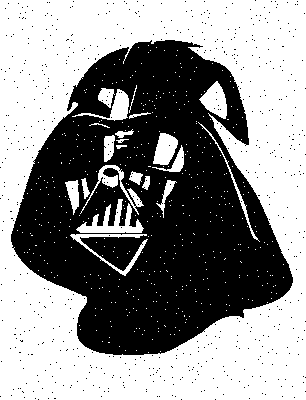
\includegraphics[width=\textwidth]{vraag3_3/uncoded_uncompressed.png}
                \caption{}
                \label{fig:3_3:uncoded_uncompressed}
            \end{subfigure}

            \begin{subfigure}{0.4\textwidth}
                \centering
                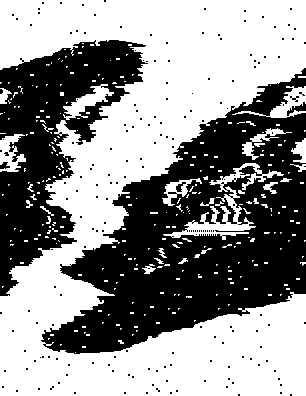
\includegraphics[width=\textwidth]{vraag3_3/compressed.png}
                \caption{}
                \label{fig:3_3:compressed}
            \end{subfigure}
            \begin{subfigure}{0.4\textwidth}
                \centering
                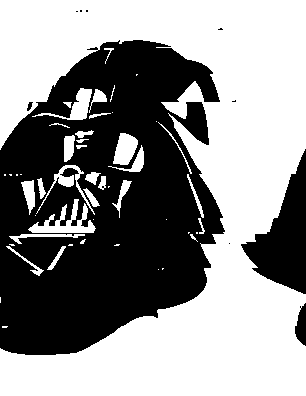
\includegraphics[width=\textwidth]{vraag3_3/coded_compressed.png}
                \caption{}
                \label{fig:3_3:coded_compressed}
            \end{subfigure}

            \caption{Figuren behorende bij vraag 3 (volledig systeem). Deze figuur
            toont respectievelijk de \emph{darthvader} figuur origineel, ongecodeerd en 
            ongecomprimeerd, gecomprimeerd met gewone huffman, gecomprimeerd met gewone
            huffman en kanaalgecodeerd.}

            \label{fig:3_3}

        \end{figure}
\end{section}
\clearpage
\begin{section}*{Overzicht Matlab bestanden}
\begin{itemize}
    \item \texttt{FakeChannel.m} : Bevat code om een kanaal dat fouten
        introduceert te simuleren. Kan ook random bit-vectoren genereren
        om de verschillende onderdelen te testen.
    \item \texttt{FrequencyCounter.m} : Bepaalt de frequenties van
        macroblokken in een afbeelding.
    \item \texttt{Vraag1\_3.m} : Geeft entropie voor macroblokken van grootte K=1..10.
    \item \texttt{Vraag1\_4.m} : Stelt Huffmancode op voor macroblokken
        van grootte K=1..10 en berekent het gemiddeld aantal
        codebits/bronsymbool met ondergrens en bovengrens. Geeft beste
        compressiefactor en de bijhorende K terug.
    \item \texttt{Vraag2\_1.m} : Stelt de generator- en checkmatrices op, 
    	alsook hun systematische versies. 
    	Heeft ook een functie om de binaire notaties te genereren van 
    	de eerste $2^n$ getallen en een functie om de minimale 
    	Hamming-afstand te bepalen.
    \item \texttt{Vraag2\_2.m} : Maakt syndroomtabel aan. Heeft zowel
        de eenvoudige manier, als de manier waarbij we eerst de
        decodeertabel opstellen.
    \item \texttt{Vraag2\_3.m} :  Simuleer het versturen van bits over
        een kanaal met bitfoutprobabiliteit $p$ en met hammingcode
        codering.
    \item \texttt{Vraag2\_6.m} : Simuleer het versturen van bits over
        een kanaal met bitfoutprobabiliteit $p$ en met productcode
        codering.
    \item \texttt{Vraag2\_7.m} : Simuleert het verzenden van de
        \texttt{darthvader.bmp} afbeelding over een transmissiekanaal
        met een kans op bitflips.
     \item \texttt{Vraag3\_3.m} : Simuleert het volledig systeem met de 3
        verschillende manieren die gevraagd werden in sectie 3.
\end{itemize}
\end{section}

\end{document}
